\section{Automated Doubling Experiments}
  \label{sec:technique}

  Our technique for performing automatic doubling experiments consists
  of two parts.  The first is a method for systematically doubling 
  the initial input schema schema, and the second is a rule for determining
  when a conclusion can be drawn from the experiment, and the experiment can be stopped. 

  \subsection{Doubling Schemas}
  \label{subsec:doubling}

  Determining worst case complexity by doubling experiment requires that
  the size of the input be doubled. A relational database
  schema is a complex artifact with many features and interrelationships. 
  This makes determining meaningful doubling rules a non-trivial task.

  % \begin{figure*}
  %   \centering
  %   \centering
  %   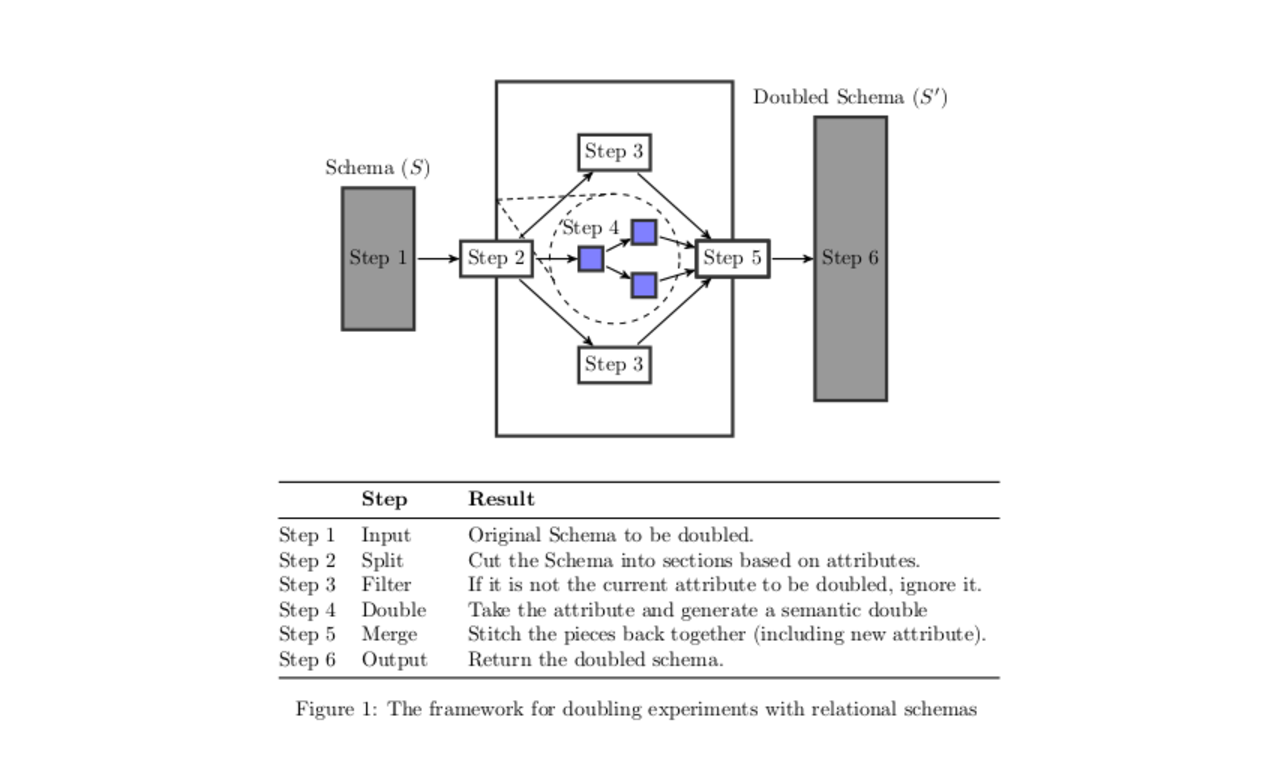
\includegraphics[width=1.25\linewidth]{../diagrams/genDouble}
  %   \caption{Multi Purpose Double Program.}
  %   \label{fig:generaldouble}
  % \end{figure*}

  A relational database schema contains tables, columns, and can contain constraints; 
  all of these items are subject to individual or grouped double. An example of
  both being \textbf{Double Tables}, which doubles all doubles but keep
  everything else constant and also \textbf{Double TablesColumns}, which
  doubles both tables and columns, but keeps everything else the same. That 
  being said, more than one algorithm for doubling is needed, but the same 
  general format is the same for all doubles.

  An example of a general semantic doubling is shown in
  Figure~\ref{fig:generaldouble}.

  \begin{figure*}
    \newcommand{\mx}[1]{\mathbf{\bm{#1}}} % Matrix command
\newcommand{\vc}[1]{\mathbf{\bm{#1}}} % Vector command

% Define the layers to draw the diagram
\pgfdeclarelayer{background}
\pgfdeclarelayer{foreground}
\pgfsetlayers{background,main,foreground}

% Define block styles used later

\tikzstyle{sensor}=[draw, fill=black!20, text width=5em,
    text centered, minimum height=2.5em,drop shadow]
\tikzstyle{ann} = [above, text width=5em, text centered]
\tikzstyle{wa} = [sensor, text width=10em, fill=red!20,
    minimum height=6em, rounded corners, drop shadow]
\tikzstyle{sc} = [sensor, text width=13em, fill=red!20,
    minimum height=10em, rounded corners, drop shadow]

% Define distances for bordering
\def\blockdist{1.5}
\def\edgedist{2.5}

\begin{tikzpicture}
    \node (wa) [wa]  {\textit{SchemaAnalyst}};
    \path (wa.west)+(-\blockdist,-1.0) node (asr1) [sensor] {Database Schema};
    \path (asr1.west)+(-\blockdist,0.0) node (doubler) [sensor] {Schema Doubler};

    \path (wa.west)+(-\blockdist,1.0) node (asr2)[sensor] {Coverage Criterion};
    \path (wa.west)+(-\blockdist,0.0) node (dots)[sensor] {Data Generator};

    \path (doubler.west)+(-\blockdist,-0.0) node (doublera) [sensor] {Schema Doubler};
    \path (dots.west)+(-2.65*\blockdist,-0.0) node (dataa) [sensor] {Data Generator};
    \path (asr2.west)+(-2.65*\blockdist,-0.0) node (criteriona) [sensor] {Coverage Criterion};
    \path (doubler.west)+(-\blockdist,-1.0) node (schemaa) [sensor] {Database Schema};



    \path (wa.east)+(\blockdist,0) node (vote) [sensor] {Test Suite};

    \path [draw, ->] (doubler.east) -- node [above] {}
    	(asr1.180);

    \path [draw, ->] (asr1.east) -- node [above] {}
        (wa.200);
    \path [draw, ->] (asr2.east) -- node [above] {}
        (wa.160);
    \path [draw, ->] (dots.east) -- node [above] {}
        (wa.180);
    \path [draw, ->] (wa.east) -- node [above] {}
        (vote.west);

    \path [draw, ->] (doublera.east) -- node [above] {}
        (doubler.west);
    \path [draw, ->] (dataa.east) -- node [above] {}
        (dots.west);
    \path [draw, ->] (criteriona.east) -- node [above] {}
        (asr2.west);
    \path [draw, ->] (schemaa.east) -| node [above] {}
        (doubler.230);

    \path (vote.east)+(\blockdist,0) node (runtime) [sensor] {Runtime Records};
    \path [draw,->] (vote.east)+(0.3,0) -- node [above]{}
    	(runtime.west);
    \path (runtime.east)+(\blockdist,0) node (runtimeo) [sensor] {Runtime Records};


     \path (vote.east)+(\blockdist,-3.165) node (convalg) [sensor] {Convergence Algorithm};
     \path [draw,->] (runtime.south) -- node [above]{}
    	(convalg.north);
     \path [draw,->] (convalg.west) -| node [above,pos=.25]{Continue Experiment}
    	(doubler.290);

	\path [draw,->] (runtime.east) -- node [above]{}
    	(runtimeo);


    \path (wa.south) +(0,-1) node (asrs) {\textit{SchemaAnalyst} Execution};

    \path (asrs.south) +(0,-1.6) node (singleexp) {Experiment Manager};

    \begin{pgfonlayer}{background}
        \path (doubler.west |- asr2.north)+(-0.3,0.6) node (a) {};
        \path (wa.south -| runtime.east)+(+0.3,-0.6) node (b) {};
        \path (runtime.east |- singleexp.east)+(+0.3,-0.3) node (c) {};

        \path[fill=yellow!20,rounded corners, draw=black!50, dashed]
            (a) rectangle (c);
        \path (asr1.north west)+(-0.2,0.2) node (a) {};

    \end{pgfonlayer}

    \begin{pgfonlayer}{background}
        \path (asr2.west |- asr2.north)+(-0.3,0.3) node (a) {};
        \path (wa.south -| wa.east)+(+0.3,-0.3) node (b) {};
        \path (vote.east |- asrs.east)+(+0.3,-0.3) node (c) {};

        \path[fill=yellow!20,rounded corners, draw=black!50, dashed]
            (a) rectangle (c);
        \path (asr1.north west)+(-0.2,0.2) node (a) {};

    \end{pgfonlayer}



\end{tikzpicture}

    \caption{Technique for conducting automatic doubling experiments.}
    \label{fig:doublingexp}
  \end{figure*}

  \subsection{Automatic Experiment}
  \label{subsec:experiment}

  To determine worst case complexity, an input $n$ is doubled until the 
  ratio $f(2n) / f(n)$ converges to a stable value. To account for random
  error, every time $n$ is doubled, $f(n)$ is recorded ten times, and the
  median time is used for calculating the ratios.  We chose
  median to minimize the effect of outliers. If mean is used instead, a
  single abnormally long run could have a large effect on the result. The overall 
  structure of the experiment is shown in Algorithm~\ref{alg:main}, and in
  Figure~\ref{fig:doublingexp}.

  This convergence checking is necessary because of the fact that worst-case
  time is only apparent for large values of $n$. If too few doubles
  are tried, then the experiment may terminate before $n$ reaches a value
  where the true worst-case time complexity is apparent. At the same time,
  for inefficient  algorithms, each additional doubling run incurs a substantial
  time overhead. For the sake of efficiently, the experiment should
  terminate as quickly as possible.
  To test for convergence, the last four ratios are compared, and the
  sum of differences between them is compared to a tolerance value. The
  convergence algorithm is shown as Algorithm~\ref{alg:convergence}.

  Another consequence of worst-case time only being apparent for large
  $n$, is that a very small initial $n$ may appear to converge to one,
  which indicates constant time. To prevent the
  experiment from incorrectly terminating given a small starting $n$, we
  require that a program under study display a ratio of one for many
  runs before judging that the ratio does in fact converge to one. Because 
  one signifies constant or logarithmic 
  time, requiring these doubles does not significantly increase the time needed
  to run the experiment, while providing assurance that a small ratio is not due
  to an insufficiently small $n$. This rule is shown in 
  Algorithm~\ref{alg:tuning}.

  \begin{algorithm}[t]
    \caption{Run Doubling Experiment}
    \begin{algorithmic}
      \WHILE{Not Convergent || N not large enough}
      \FOR{$\mathit{trials}$}
      \STATE Run Test
      \ENDFOR
      \STATE Double Schema
      \ENDWHILE
    \end{algorithmic}
    \label{alg:main}
  \end{algorithm}

  \begin{algorithm}[t]
    \caption{Convergent}
    \begin{algorithmic}
      \STATE difference $= |(r_4 - r_3) + (r_3 -r_2) + (r_2 - r_1)|$
      \IF{difference $< \mathit{differanceTolerance}$}
      \RETURN Ratio is convergent
      \ELSE
      \RETURN Ratio is not convergent
      \ENDIF
    \end{algorithmic}
    \label{alg:convergence}
  \end{algorithm}

  \begin{algorithm}[t]
    \caption{N Large Enough}
    \begin{algorithmic}
      \IF{ratio $\approx 1$}
      \IF{number of doubles $< \mathit{doublesTolerance}$}
      \RETURN N is not large enough
      \ENDIF
      \ENDIF
      \RETURN N is large enough
    \end{algorithmic}
    \label{alg:tuning}
  \end{algorithm}
